% \documentclass[notes=only]{beamer}
\documentclass{beamer} 

% Deutsch
\usepackage[german]{babel} % deutsch und deutsche Rechtschreibung
\usepackage[utf8]{inputenc} % Unicode Text 
\usepackage[T1]{fontenc} % Umlaute und deutsches Trennen
\usepackage{textcomp} % Euro
% \usepackage[hyphens]{url}
\usepackage{emptypage} % Wirklich leer bei leeren Seiten
\usepackage{listings}
\usepackage{xcolor}
\usetheme[]{antibes}

\definecolor{codegreen}{rgb}{0,0.6,0}
\definecolor{codegray}{rgb}{0.5,0.5,0.5}
\definecolor{codepurple}{rgb}{0.58,0,0.82}
\definecolor{backcolour}{rgb}{0.95,0.95,0.92}

\lstdefinestyle{mystyle}{
    backgroundcolor=\color{backcolour},   
    commentstyle=\color{codegreen},
    keywordstyle=\color{magenta},
    numberstyle=\tiny\color{codegray},
    stringstyle=\color{codepurple},
    basicstyle=\ttfamily\footnotesize,
    breakatwhitespace=false,         
    breaklines=true,                 
    captionpos=b,                    
    keepspaces=true,                 
    numbers=left,                    
    numbersep=5pt,                  
    showspaces=false,                
    showstringspaces=false,
    showtabs=false,                  
    tabsize=2
}
\lstset{style=mystyle}

\AtBeginSubsection[]{
  \begin{frame}
  \vfill
  \centering
  \begin{beamercolorbox}[sep=8pt,center,shadow=true,rounded=true]{title}
    \usebeamerfont{title}\insertsubsectionhead\par%
  \end{beamercolorbox}
  \vfill
  \end{frame}
}

\AtBeginSection[
  {\frame<beamer>{\frametitle{Outline}   
    \tableofcontents[currentsection,currentsubsection]}}%
]%
{
  \frame<beamer>{ 
    \frametitle{Übersicht}   
    \tableofcontents[currentsection]}
}

\usepackage[yyyymmdd]{datetime}
\renewcommand{\dateseparator}{--}
%Information to be included in the title page:
\title{Smartbit}
\author{Marius Cerwenetz\\ \vspace{1cm}
\scriptsize Betreuung:  Prof. Dr. Peter Barth, Prof. Dr. Jens-Matthias Bohli}
\institute{Institut für Softwaretechnik und Datenkommunikation}
\date{\today}
\logo{
\includegraphics[width=0.1\textwidth]{images/hsma_logo.pdf}}

\beamertemplatenavigationsymbolsempty

\begin{document}

\frame{\titlepage}

\addtobeamertemplate{navigation symbols}{}{%
    \usebeamerfont{footline}%
    \usebeamercolor[fg]{footline}%
    \hspace{1em}%
    \insertframenumber/\inserttotalframenumber
}
\logo{}

\setcounter{tocdepth}{1}
\begin{frame}
\frametitle{Agenda}
% \tableofcontents[pausesections]
\tableofcontents

\end{frame}

\section{Einführung}

\begin{frame}
    \frametitle{Schwierigkeiten beim Programmierenlernen}
    \begin{itemize}
        \item Semantik
        \item Grundkonzepte
        \item Theoretische Übungsaufgaben
    \end{itemize}
\end{frame}

\begin{frame}
    \frametitle{Microcontroller als Alternative}
    \begin{itemize}
        \item Interaktivität durch Sensoren
        \item Ausgabemöglichkeiten (LEDs, Piepser, Aktoren)
        \item Ausprobieren
    \end{itemize}

    \begin{alertblock}{Nachteile}
        \begin{itemize}
            \item Beschaffung
            \item Peripherie
        \end{itemize}
    \end{alertblock}
\end{frame}



\begin{frame}
    \frametitle{Smartphones für interaktive Lernaufgaben}
    \begin{itemize}
        \item Hohe Verfügbarkeit
        \item Keine Verdrahtungsfehler
        \item Unabhängige Spannungsversorgung
        \item Zahlreiche Sensoren bereits integriert
        \item Drahtlose Verbindungstechnologien (WLAN, Bluetooth, UMTS/LTE)
    \end{itemize}
\end{frame}

\begin{frame}
    \frametitle{Technische Hürden}
    \begin{alertblock}{Voraussetzungen}
        \begin{itemize}
            \item Anbindung in Programmierumgebungen
            \item Smartphone-App
        \end{itemize}
    \end{alertblock}
    \begin{block}{Lösungsansatz}
        Software-Lösung zur Kommunikation mit dem Smartphone
    \end{block}
\end{frame}

\section{Anforderungen}
\begin{frame}
    \frametitle{Vorgehen}
    \begin{itemize}
        \item Beispielaufgaben für µC und Smartphones
        \item Anforderungen ableiten
    \end{itemize}
\end{frame}

\begin{frame}
    \frametitle{Beispielaufgaben}
    \begin{itemize}
        \item Disco
        \item Würfeln
        \item Diebstahl-Alarm
        \item Dreh-Zähler
    \end{itemize}
\end{frame}

\begin{frame}
    \frametitle{Anforderungen}
    \begin{itemize}
        \item UI-Elemente der Beispielaufgaben
        \item Sensordatenübermittlung
        \item Geringe Latenzen / Hohe Interaktivität
    \end{itemize}
\end{frame}

\section{Smartbit}
\begin{frame}
    \frametitle{Aufbau der Smartbit-Lösung}
    \begin{columns}
        \begin{column}{0.3\textwidth}
            \centering
            
\includegraphics[width=5em]{images/lib.pdf}
            Bibliothek
        \end{column}
        \begin{column}{0.3\textwidth}
            \centering
            
\includegraphics[width=5em]{images/server.pdf}
            Kontrollanwendung
        \end{column}
        \begin{column}{0.3\textwidth}
            \centering
            
\includegraphics[width=5em]{images/android.pdf}
            Android-App
        \end{column}
    \end{columns}
\end{frame}

\begin{frame}[fragile]
    \frametitle{Bibliothek}
    Funktionsaufrufe für Sensorwerte und Ausgaben.
    \begin{columns}
        \begin{column}{0.3\textwidth}
            Einbindbar in:
            \begin{itemize}
                \item C
                \item Java
                \item Python
            \end{itemize}
        \end{column}
        \begin{column}{0.6\textwidth}
            \begin{lstlisting}[language=python]
from  smartbit import Phone
p = Phone()
accel = p.get_x_accelo()
p.write_text("hallo")
            \end{lstlisting}
        \end{column}
    \end{columns}
    
   
\end{frame}

\begin{frame}
    \frametitle{Smartphone-App}
    \centering
    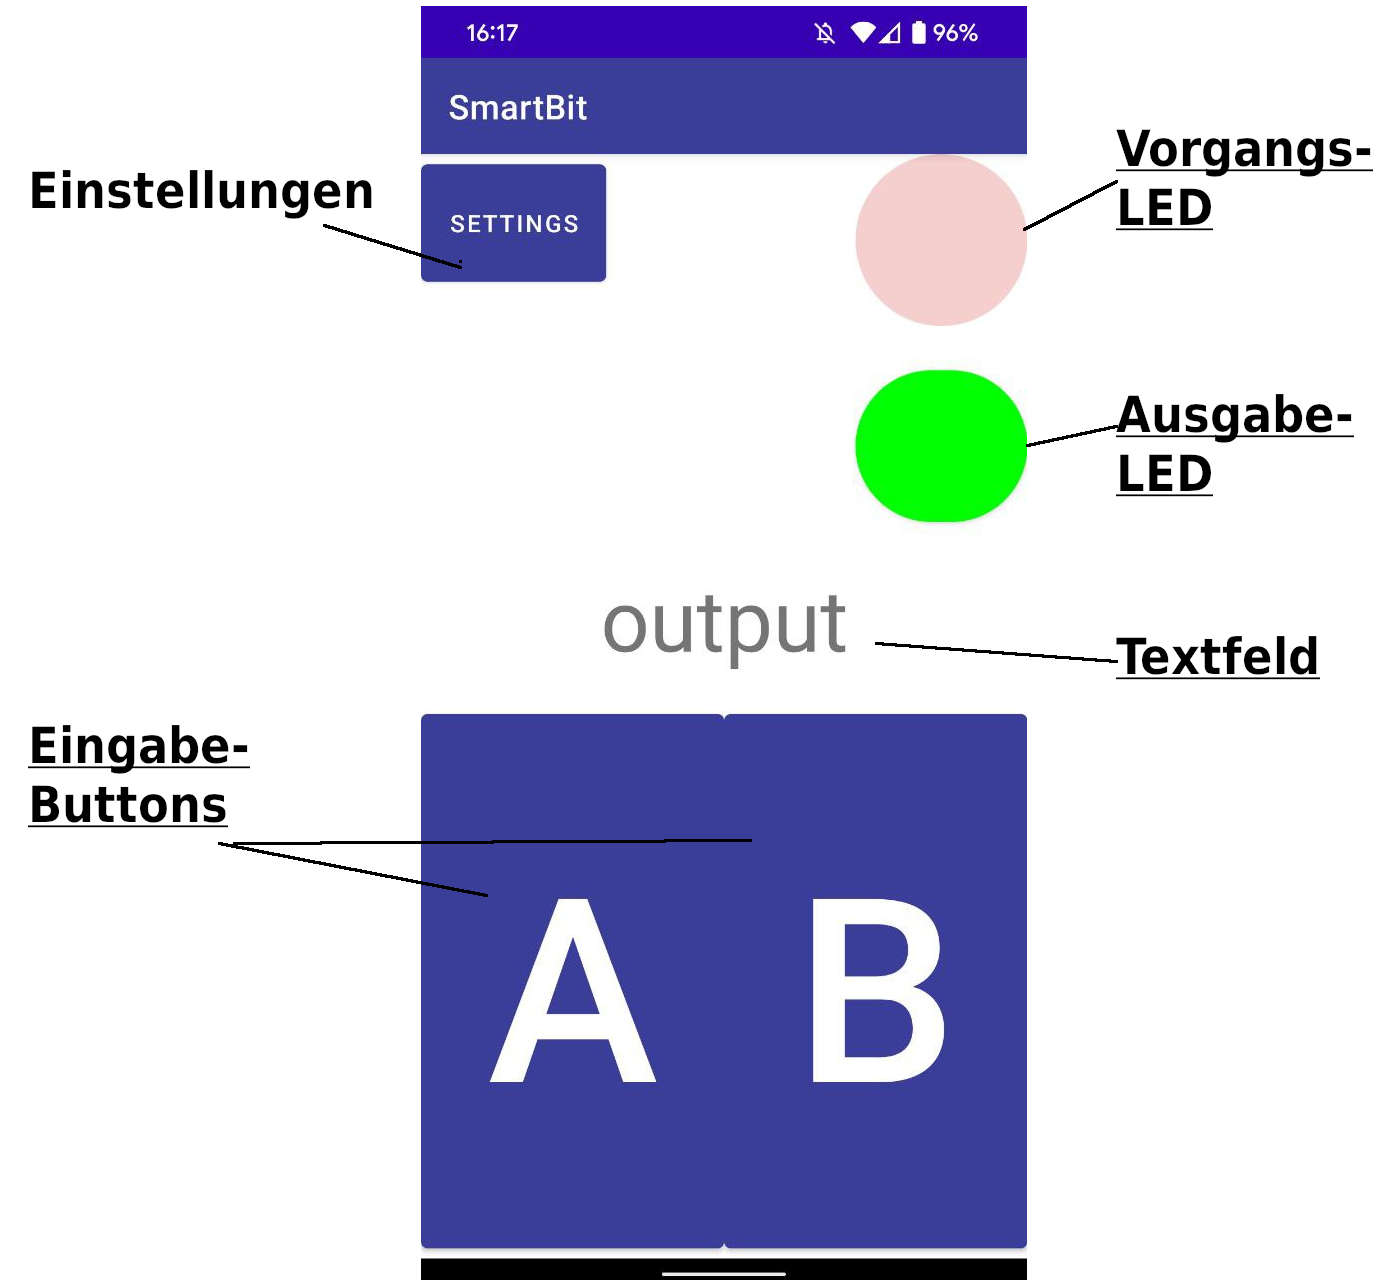
\includegraphics[height=0.8\textheight]{images/app_initial.png}
\end{frame}

\begin{frame}[fragile]
    \frametitle{Kontrollanwendun}
    \begin{center}
    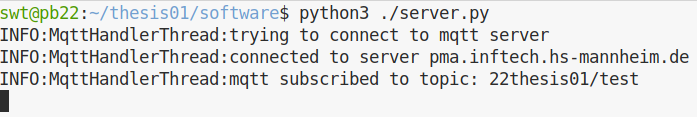
\includegraphics[width=0.8\textwidth]{images/middleware.png}
    \end{center}
\end{frame}

\section{Architektur}
\subsection{Übersicht der Gesamtarchitektur}
\begin{frame}
    \frametitle[]{Architektur}
    \centering
    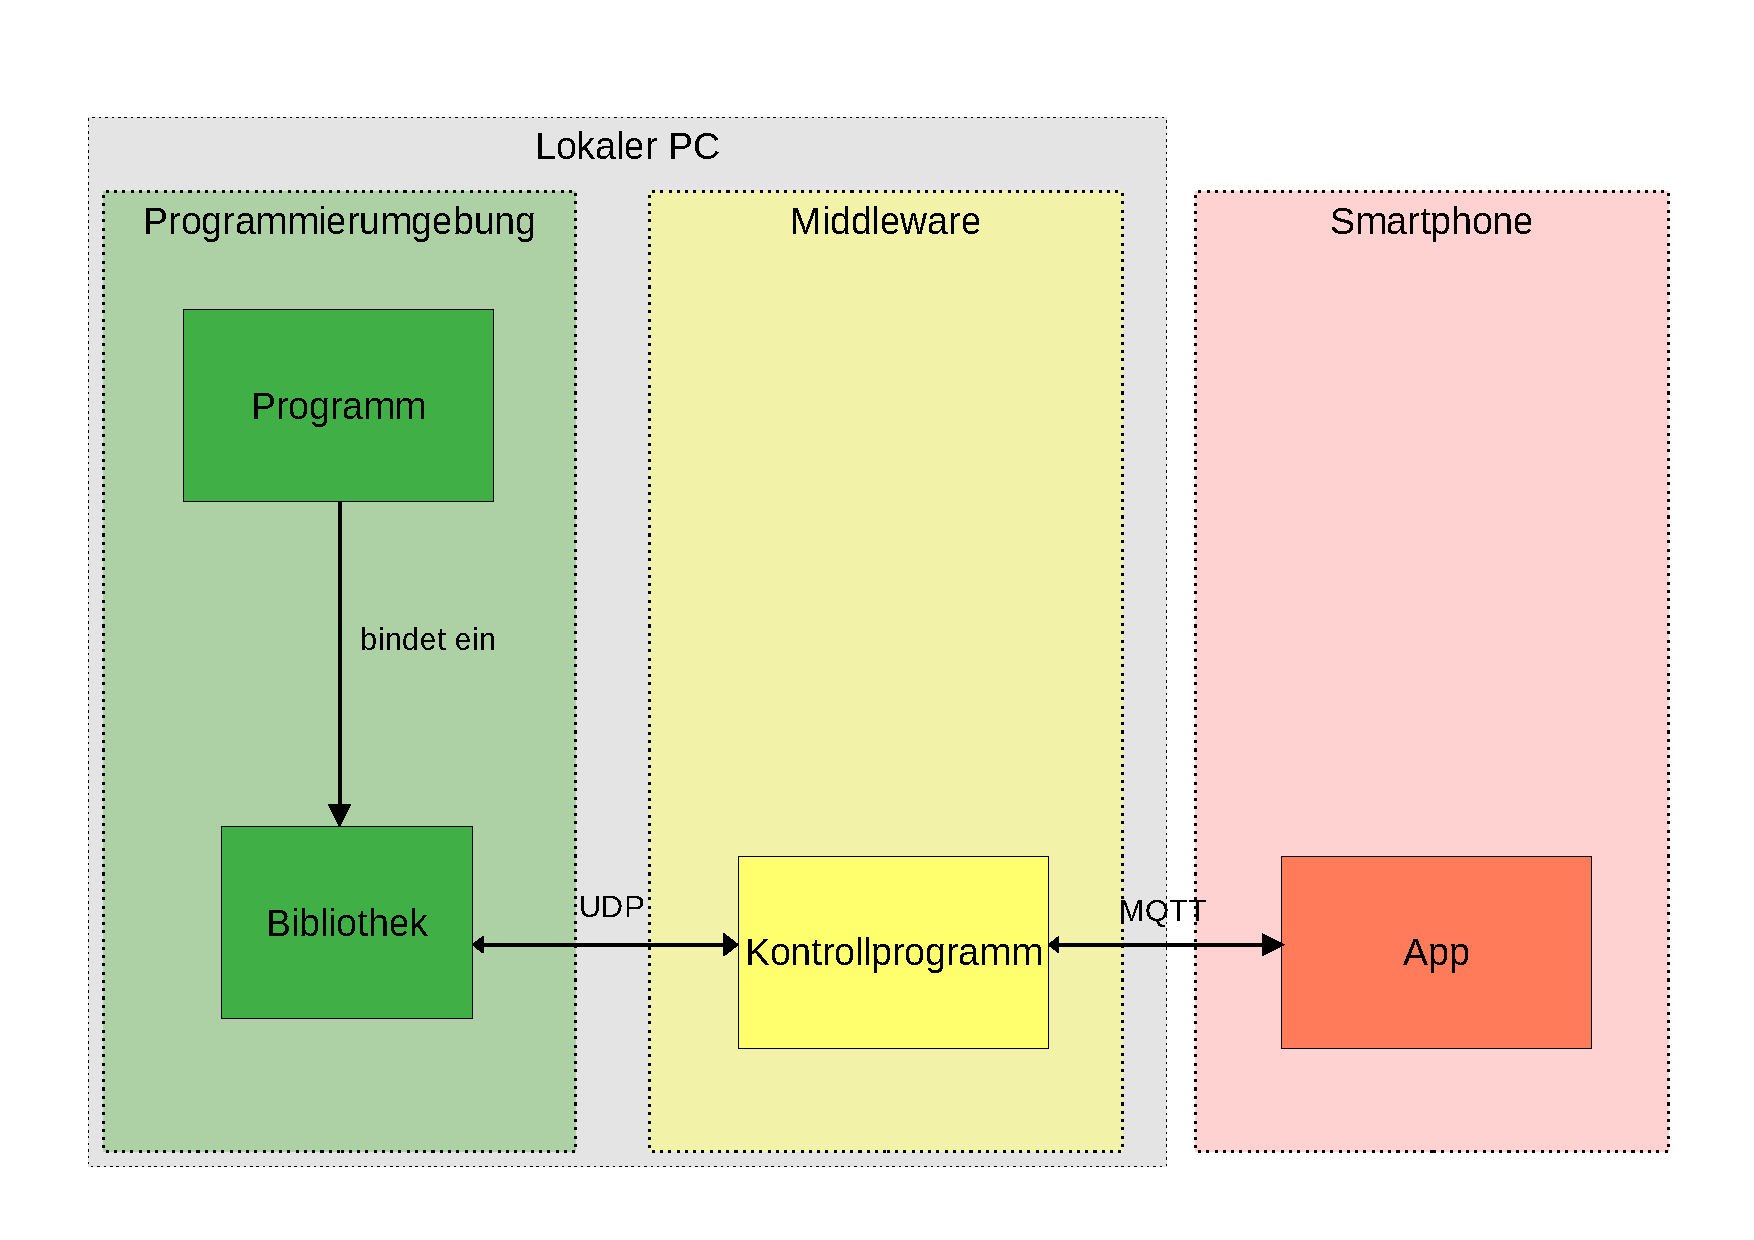
\includegraphics[width=0.9\textwidth]{images/framework.pdf}
\end{frame}

\subsection*{Nachrichten}
\begin{frame}
    \frametitle[]{Nachrichtenformate}
    \begin{columns}
        \begin{column}{0.5\textwidth}
        Requests
            \begin{itemize}
                \item update\_request
                \item sensor\_request
                \item rpc\_request
            \end{itemize}
        \end{column}
        
        \begin{column}{0.5\textwidth}
        Responses
        \begin{itemize}
            \item sensor\_response
            \item rpc\_response
        \end{itemize}
        \end{column}
    \end{columns}

        
\end{frame}

\begin{frame}[fragile]
    \frametitle{Beispielnachricht - Neuer Sensorwert}
    \begin{lstlisting}[language=python]
{
    "type": "update_request",
    "sensor_type": "",
    "sensor_value": ""
}
\end{lstlisting}
\end{frame}

\begin{frame}
    \frametitle[]{Konfigurationsdateien}
    \begin{itemize}
        \item protocol.json
        \item config.json
        \item Dezentral auf alle drei Komponenten verteilt
    \end{itemize}
\end{frame}

\subsection{Bibliothek}

\begin{frame}
    \frametitle{Aufgaben}
    Funktionen für:
    \begin{itemize}
        \item Ausgabemöglichkeiten
        \item Sensorwertabfragen
    \end{itemize}
\end{frame}

\begin{frame}
    \frametitle[]{Funktionsweise}
    \begin{itemize}
        \item Stub-Funktionen
        \item Local-Loopback
        \item UDP, Port 5006
        \item CJSON und JSON for Java
    \end{itemize}
\end{frame}

\begin{frame}[fragile]
    \frametitle{Beispiel-Funktion: Vibration}
    \begin{lstlisting}[language=python]
def vibrate(self, time : int):
"vibrates phone for time miliseconds"
def _vibrate(self):
    rpc_message = JsonMessagesWrapper.get_rpc_request(command="vibrate", value=str(time))
    self._sendMessage(rpc_message)
threading.Thread(target=_vibrate, args=(self, )).start()
    \end{lstlisting}
\end{frame}

\subsection{Smartphone-App}

\begin{frame}
    \frametitle{Aufgaben}
    \begin{itemize}
        \item Sensorwert-Übermittlung
        \item Ausgeben von Ausgabeanfragen
    \end{itemize}
\end{frame}

\begin{frame}
    \frametitle[]{Funktionsweise}
    SensorEventListener
    \begin{itemize}
        \item Neue Sensormessdaten
        \item Übermittlung an Kontrollanwendung
    \end{itemize}
    \vspace{1cm}
    MessageListener
    \begin{itemize}
        \item Warten auf Nachrichten
        \item Reaktion Ausgabe
        \item Ggf. RPC-Antwort
    \end{itemize}

\end{frame}

\begin{frame}
    \frametitle[]{Sensoren}
    \begin{columns}
        \begin{column}{0.5\textwidth}
            \begin{itemize}
                \item Beschleunigungssensor
                \item Gyroskop
                \item Annäherungssensor
            \end{itemize}
        \end{column}
        \begin{column}[]{0.5\textwidth}
            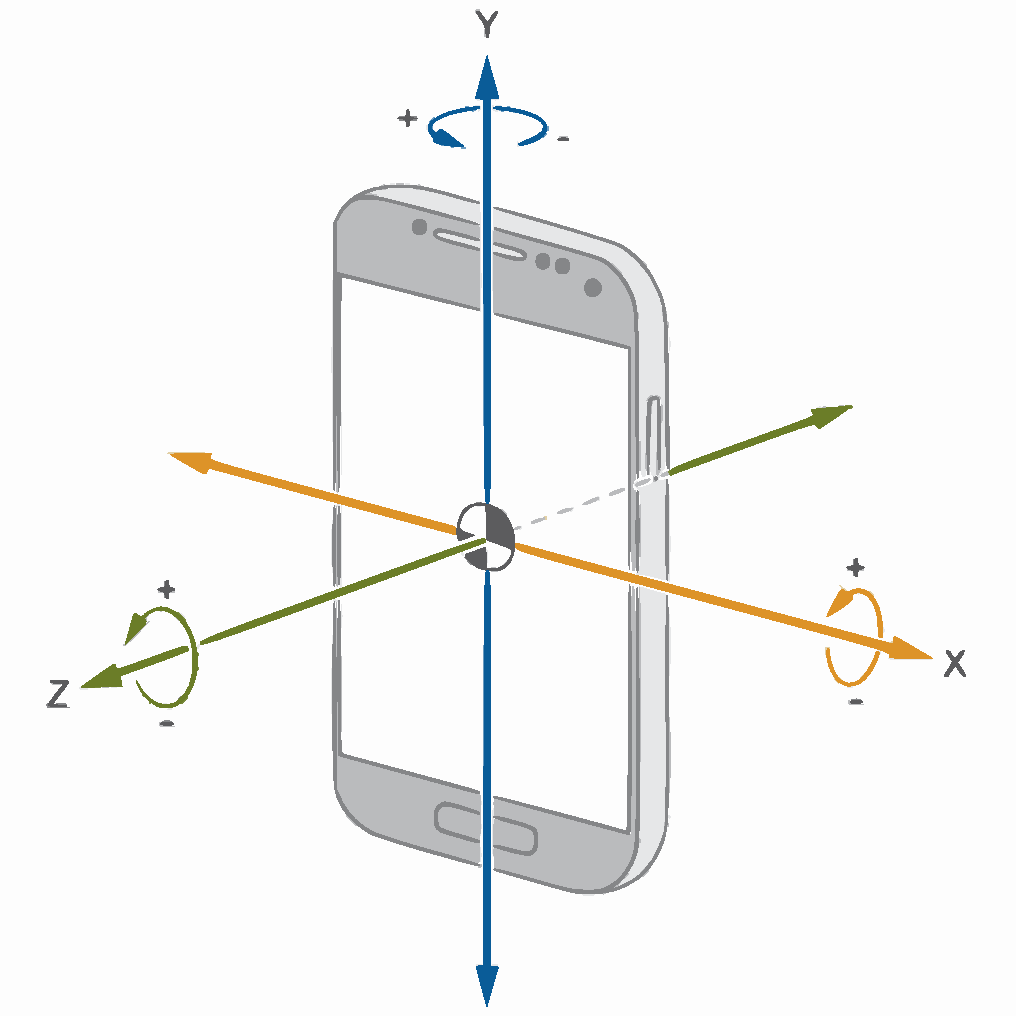
\includegraphics[width=\textwidth]{images/android_axes.pdf}
        \end{column}
    \end{columns}
\end{frame}


\subsection{Kontrollanwendung}
\begin{frame}
    \frametitle[]{Aufgaben}
    Aufgaben:
    \begin{itemize}
        \item Sensormesswerte annehmen und speichern
        \item Sensor-Anfragen beantworten
        \item RPC-Anfragen weiterleiten
        \item RPC-Antworten weiterleiten
    \end{itemize}
\end{frame}

\begin{frame}
\frametitle[]{Funktionsweise}
\begin{itemize}
    \item Mehrere Threads
    \item Kommunikation per MQTT und UDP
    \item UDP Port 5005
    \item Thread-Kommunikation durch Python-Queues
\end{itemize}
\end{frame}

\begin{frame}
\frametitle[]{Aufbau der Kontrollanwendung}
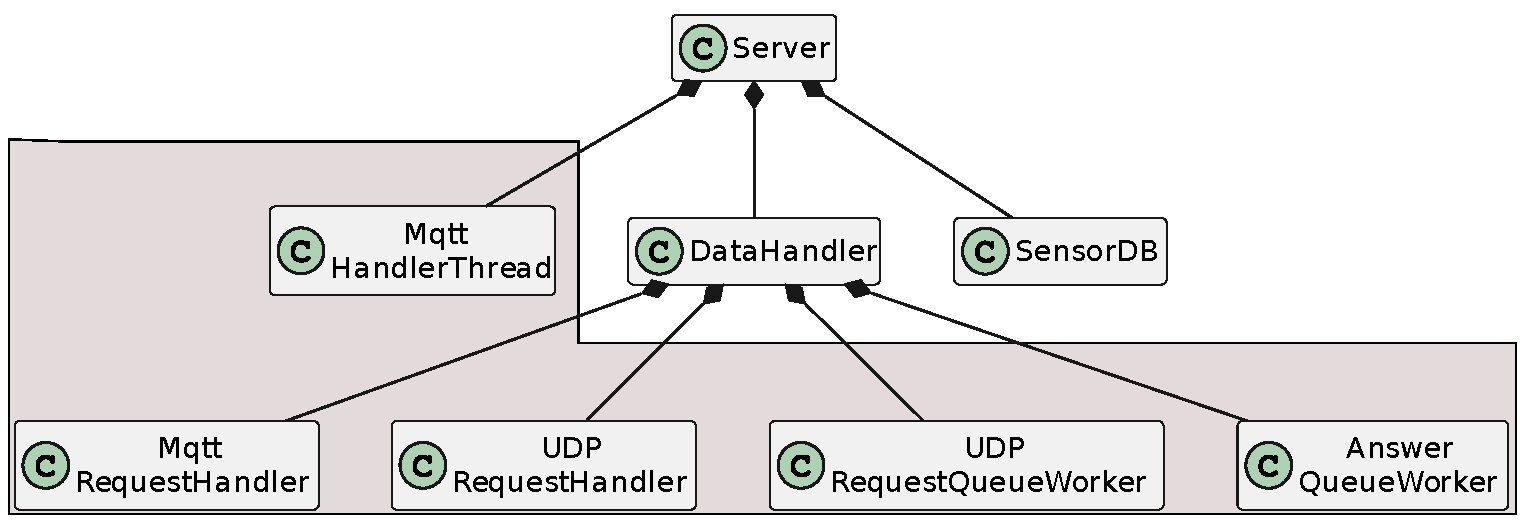
\includegraphics[width=\textwidth]{images/ServerUml.pdf}
\end{frame}


\section{Evaluation}
\subsection{Latenzen}

\begin{frame}
    \frametitle{Kontext}

    \begin{columns}
        \begin{column}{0.5\textwidth}
            Szenarios
            \begin{enumerate}
                \item SWT-Labor
                \item Zuhause
                \item Per VM
            \end{enumerate}
        \end{column}
        \begin{column}{0.5\textwidth}
            Nebenbedingungen
            \begin{itemize}
                \item Umlaufzeit
                \item Unter Last
                \item Python
            \end{itemize}
        
        \end{column}
    \end{columns}
\end{frame}
\begin{frame}
    \frametitle[]{Latenzen}
    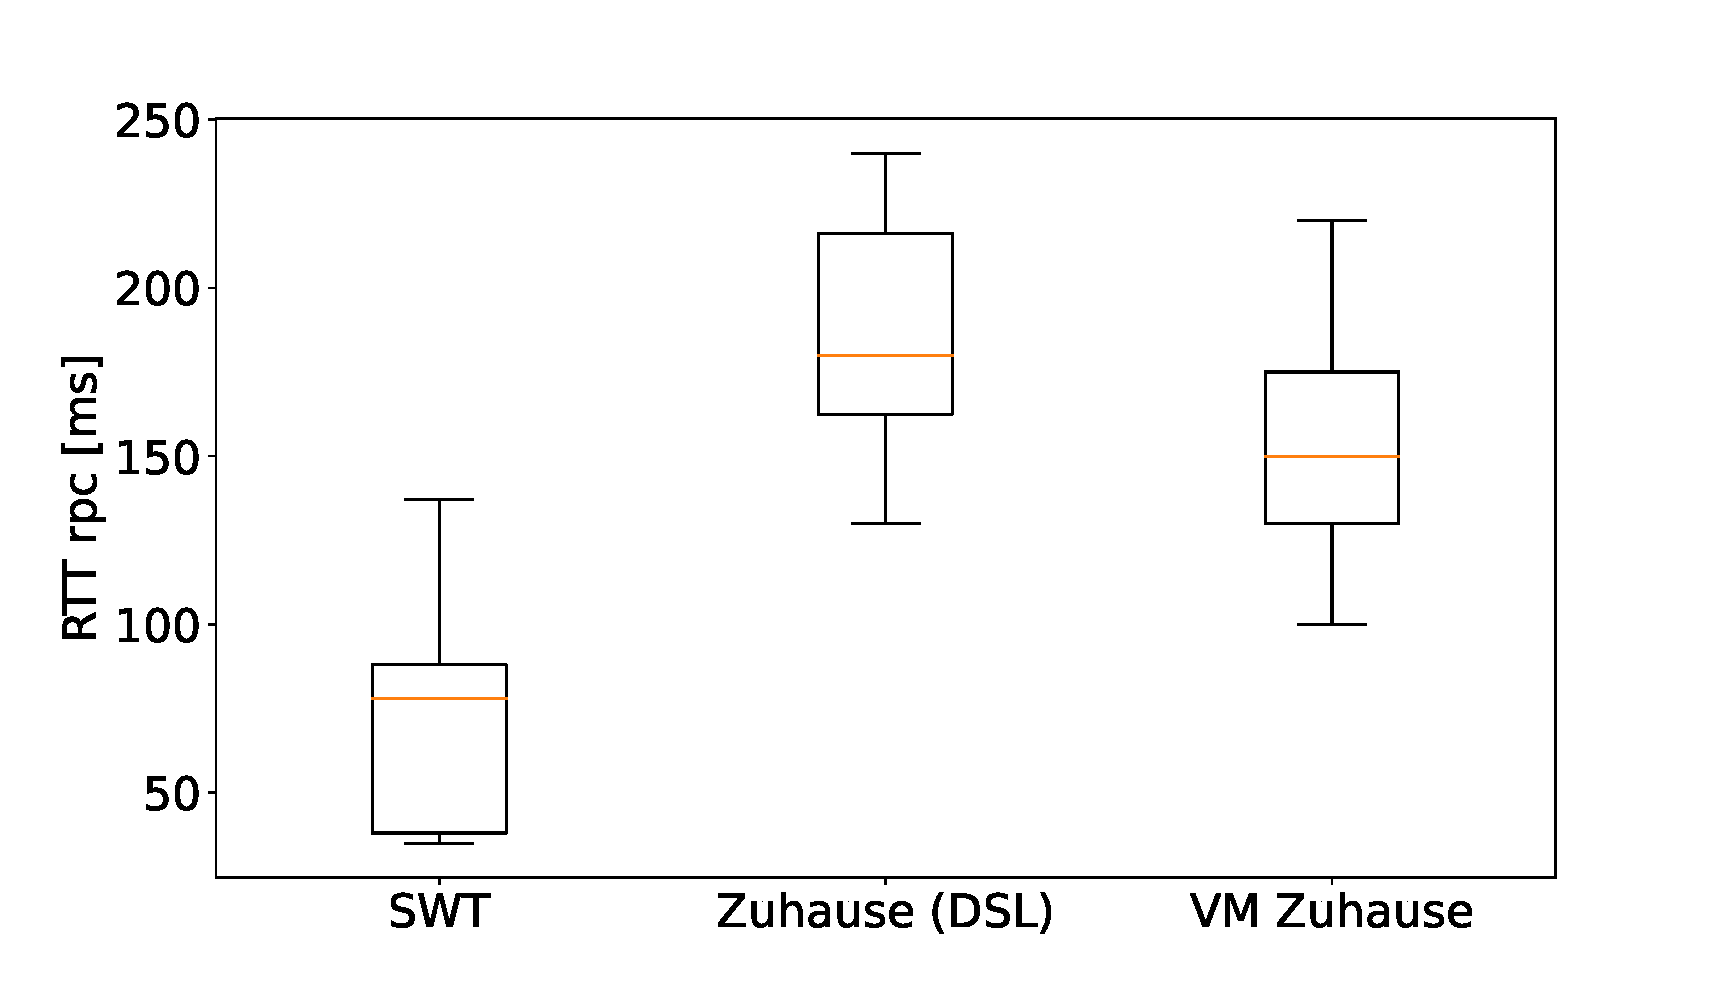
\includegraphics[width=\textwidth]{images/latencies.pdf}
\end{frame}


\begin{frame}
    \frametitle[]{Sonstiges}
    \begin{itemize}
        \item Portabilität
        \item Latenzverschleierung durch Caching
        \item Transparenter Ablauf durch Logging
    \end{itemize}
\end{frame}
\section{Fazit und Ausblick}
\begin{frame}
    \frametitle[]{Fazit}
    \begin{itemize}
        \item Alle Anforderungen implementiert
        \item JSON-Parser
        \item Latenzzeiten tolerabel
        \item Objekt-Orientierung
        \item Verfügbarkeit
    \end{itemize}
\end{frame}
\begin{frame}
    \frametitle[]{Ausblick}
    \begin{itemize}
        \item QR-Code für Konfigurationen
        \item Mehrere Sensorwerte zwischenspeichern
        \item Burst-Mode / Selektive Sensormessung
        \item Group-Sessions
    \end{itemize}
\end{frame}

\begin{frame}
    \frametitle{Ende}
    \vfill
    \centering
    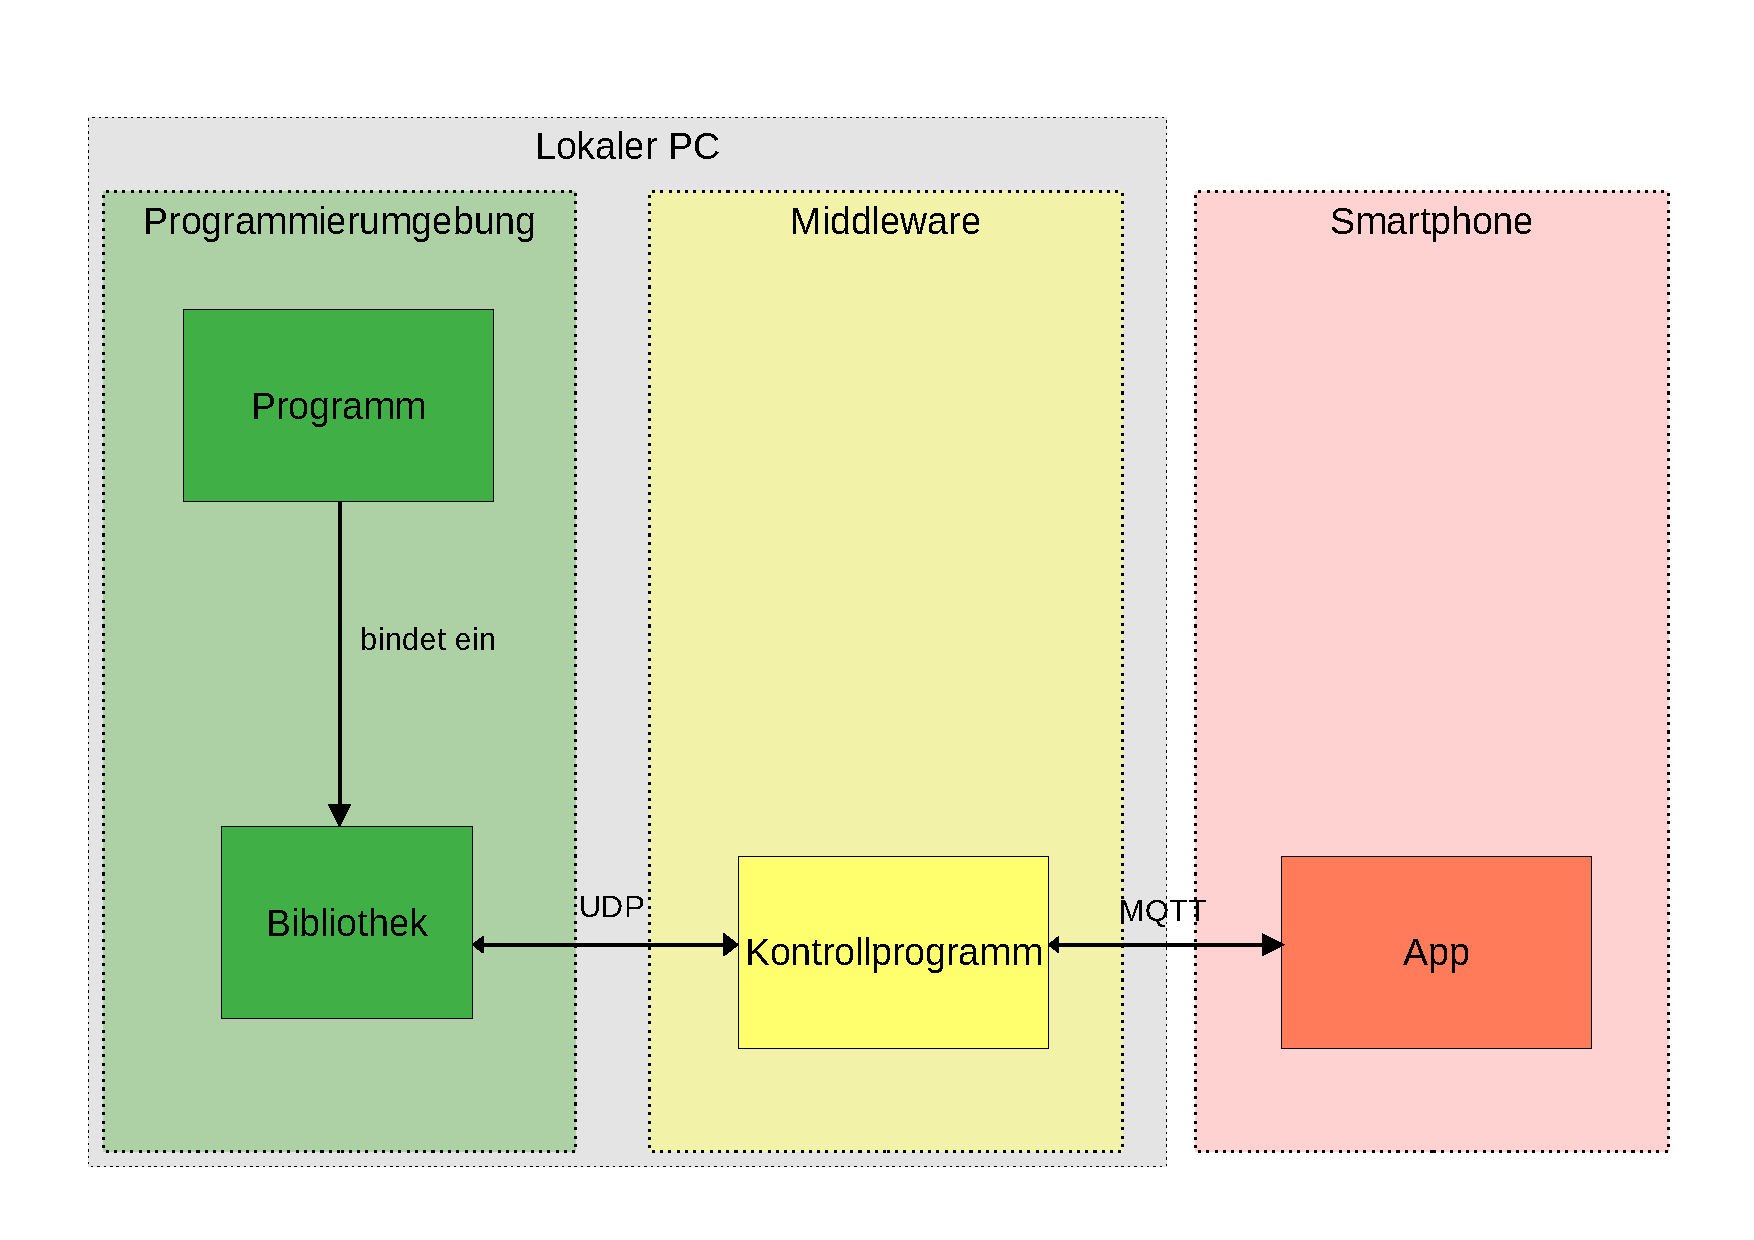
\includegraphics[width=0.9\textwidth]{images/framework.pdf}
\end{frame}

\begin{frame}
    \vfill
    \centering
    \begin{beamercolorbox}[sep=8pt,center,shadow=true,rounded=true]{title}
      \usebeamerfont{title}Demo
    \end{beamercolorbox}
    \vfill
    \end{frame}

\end{document}